%% LyX 2.3.6.1 created this file.  For more info, see http://www.lyx.org/.
%% Do not edit unless you really know what you are doing.
\documentclass[english]{article}
\usepackage[T1]{fontenc}
\usepackage[latin9]{inputenc}
\usepackage{geometry}
\geometry{verbose,tmargin=2.5cm,bmargin=2.5cm,lmargin=2.5cm,rmargin=2.5cm}
\usepackage{amsmath}
\usepackage{graphicx}

\makeatletter

%%%%%%%%%%%%%%%%%%%%%%%%%%%%%% LyX specific LaTeX commands.
%% Because html converters don't know tabularnewline
\providecommand{\tabularnewline}{\\}

\makeatother

\usepackage{babel}
\begin{document}
{[}SPLIT\_HERE{]}
\begin{enumerate}
\item \textbf{{[}DHS/PRELIM/9597/2015/P1/Q1{]} }

The coming General Election will see 28481 voters in the MacPherson
Single Member Constituency (SMC) voting for their Member of Parliament
(MP). The data file \texttt{ELECTION.txt} contains the simulated voting
results, with A, B, C and V representing votes for the political parties
National Solidarity Party, People Action Party and Workers' Party,
as well as void votes respectively. 

\subsection*{Task 1.1}

Determine the winner and the voting statistics (correct to 1 decimal
place) for this SMC. Your output should look like the following: 

Sample output: 

\noindent %
\noindent\begin{minipage}[t]{1\columnwidth}%
\texttt{Results for the Electoral Division of MacPherson }

\texttt{PAP 58.7\%}

\texttt{WP 37.5\%}

\texttt{NSP 2.6\% }

\texttt{Void 1.2\%}

\texttt{Winner is PAP }%
\end{minipage}

\subsection*{Evidence 1 }

Program code. \hfill{}{[}7{]}

\subsection*{Evidence 2}

Screenshot.\hfill{} {[}1{]}

\subsection*{Task 1.2}

In the event of a tie, the parties tied will enter into a revoting
exercise. For example, if there is a tie between PAP and WP, return
the message \textquotedbl\texttt{Revote between PAP and WP}\textquotedbl . 

Write program code to generate a text file \texttt{TIE.txt} with approximately
3\% void votes, 7\% votes for NSP and a tie between PAP and WP. Test
your program with your generated \texttt{TIE.txt}. 

\subsection*{Evidence 3 }

Program code.\hfill{} {[}6{]}

\subsection*{Evidence 4 }

Screenshot. \hfill{}{[}1{]}

{[}SPLIT\_HERE{]}
\item \textbf{{[}DHS/PRELIM/9597/2015/P1/Q2{]} }

You are provided with the registration dates and email addresses of
participants who registered for an event in the text file \texttt{PARTICIPANTS.txt}.
Unfortunately, some participants registered more than once. 

\subsection*{Task 2.1 }

Write program code to remove duplicate entries and generate the final
participant list in alphabetical email order. If a participant registered
more than once, take the last registered record as the final entry.
Return also a count of duplicate entries removed. 

Sample output:

\noindent %
\noindent\begin{minipage}[t]{1\columnwidth}%
\texttt{ali@yahoo.com,03-05-2015}

\texttt{dave@savetheworld.org,05-05-2015 }

\texttt{james007@bond.uk,07-05-2015}

\texttt{limahseng@gmail.com,01-05-2015 }

\texttt{mary\_ong@m1.com.sg,05-05-2015 }

\texttt{zorro@outlook.com,30-04-2015 }

\texttt{3 duplicate entries removed.}%
\end{minipage}

\subsection*{Evidence 5 }

Program code. \hfill{}{[}4{]}

\subsection*{Evidence 6 }

Screenshot.\hfill{} {[}1{]}

\subsection*{Task 2.2 }

Some email addresses may be entered wrongly. Using first principles,
write a Boolean function \texttt{Valid\_Email(email)} to determine
if an email address is valid. Design test cases to thoroughly test
the working of your function code. 

\subsection*{Evidence 7 }

Program code.\hfill{} {[}6{]}

\subsection*{Evidence 8}

Test data with purpose and corresponding screenshots. \hfill{}{[}4{]}

{[}SPLIT\_HERE{]}
\item \textbf{{[}DHS/PRELIM/9597/2015/P1/Q3{]} }

International Standard Book Number (ISBN) is a unique number assigned
to each edition of a book. It has two formats: ISBN-10 and ISBN-13.
The former is used before 1 Jan 2007 and the latter after that. Examples
of valid ISBNs are 020103803X and 978-1-284-05591-7. The last digit
is the check digit and is computed as follows:

\textbf{ISBN check digit (10 digits) - mod 11 algorithm} 
\begin{itemize}
\item Each digit starting from left to right is assigned a weight from 1
to 9. Each digit is multiplied by its position weight. The sum of
products modulo 11 gives a remainder between 0 and 10. If the remainder
is 10, the check digit is the roman numeral X, else the check digit
is the remainder.
\item \textbf{Example ISBN-10: 0-07-063546-3 }

$(0\times1)+(0\times2)+(7\times3)+(0\times4)+(6\times5)+(3\times6)+(5\times7)+(4\times8)+(6\times9)=190$
\item $190\mod11=3$
\item Hence 3 is the check digit. 
\end{itemize}
\textbf{ISBN check digit (13 digits) - mod 10 algorithm}
\begin{itemize}
\item Each digit starting from the left to right is multiplied by 1 or 3
alternatively. The sum of the products modulo 10 gives a remainder
between 0 to 9. If the remainder is nonzero, subtract this from 10
to get the check digit, else the check digit is 0. 
\item Example ISBN-13: 978-0-07-063546-3 

$1\times9+3\times7+1\times8+3\times0+1\times0+3\times7+1\times0+3\times6+1\times3+3\times5+1\times4+3\times6=117$
\item $117\mod10=7$
\item $10-7=3$ 
\item Hence 3 is the check digit. 
\end{itemize}

\subsection*{Task 3.1}

Write a function \texttt{ISBN\_Check\_Digit(isbn)} which generates
the check digit for a given ISBN-10 or ISBN-13 number. 

\subsection*{Evidence 9 }

Program code. \hfill{}{[}5{]}

\subsection*{Evidence 10 }

Screenshots (1 for ISBN-10 and 1 for ISBN-13)\hfill{} {[}2{]}

\subsection*{Task 3.2 }

Write a function \texttt{Valid\_ISBN(isbn)} which calls your \texttt{ISBN\_Check\_Digit(isbn)}
function in Task 3.1 to determine if a given ISBN-10 or ISBN-13 number
is valid. 

\subsection*{Evidence 11 }

Program code. \hfill{}{[}4{]}

\subsection*{Evidence 12 }

Screenshots for appropriately generated ISBN-10 and ISBN-13 numbers.\hfill{}
{[}2{]}

An ISBN-10 number can be converted to its ISBN-13 equivalent by prefixing
'978' to the ISBN-10 number and then calculating the check digit using
the ISBN-13 algorithm. 

\subsection*{Task 3.3 }

Write a function \texttt{ISBN10\_To\_ISBN13(isbn)} to convert an ISBN-10
number to its ISBN13 equivalent.

\subsection*{Evidence 13 }

Program code. \hfill{}{[}3{]}

\subsection*{Evidence 14 }

Screenshot of output for ISBN-10 number 1904467520. \hfill{}{[}1{]}

\subsection*{Task 3.4}

Write a function \texttt{ISBN13\_To\_ISBN10(isbn)} to convert an ISBN-13
number to its ISBN10 equivalent.

\subsection*{Evidence 15 }

Program code. \hfill{}{[}4{]}

\subsection*{Evidence 16 }

Screenshot of output for ISBN-13 number 9780748740468. \hfill{} {[}1{]}

A small library wishes to store its book collection details using
a random file organisation. It currently holds 200 books but wishes
to expand its collection by about 10\% every year. To resolve collisions,
it decides to use double hashing which minimises clustering. For a
start, assume that this file organisation will be maintained for 3
years. 

\subsection*{Task 3.5 }

Devise and implement a suitable double hashing strategy \texttt{Hash\_Key(isbn)}.
Annotate your strategy using program comments. 

\subsection*{Evidence 17}

Program code with comments. \hfill{}{[}5{]}

\subsection*{Task 3.6}

Write program code to generate an appropriate number of ISBNs to the
random text file \texttt{LIBRARY.txt} which will cater to the library's
collection growth over 3 years. Include \texttt{Insert\_Book(isbn)}
and \texttt{Lookup\_Book(isbn)} functions to insert a book and lookup
a book respectively. 

\subsection*{Evidence 18}

Program code. \hfill{} {[}8{]}

\subsection*{Evidence 19 }

Screenshots showing the insertion and lookup of one non-collided record
and one collided record. \hfill{}{[}4{]}

\subsection*{Evidence 20 }

Separate printout of \texttt{LIBRARY.txt} after insertion of all generated
records. \hfill{} {[}2{]}

{[}SPLIT\_HERE{]}
\item \textbf{{[}DHS/PRELIM/9597/2015/P1/Q4{]} }

You are tasked to maintain a binary search tree for optimal search
efficiency. Each node of the binary search tree contains a unique
identifier (productid) and a reference to a linked list which holds
individual order details for that product. For simplicity, orderid
will suffice. 

\subsection*{Task 4.1 }

Using object-oriented programming, implement the above binary search
tree with its associated class methods (\texttt{insert()}, \texttt{search()}
and \texttt{inorder()}). 

\subsection*{Evidence 21}

Program code for binary search tree with 8 products inserted, 3 of
which has at least 2 orders. \hfill{}{[}8{]}

\subsection*{Evidence 22}

Screenshot of output of inorder traversal (product and order information).
\hfill{} {[}2{]}

\subsection*{Task 4.2 }

Write a support class method most\_popular() to determine the best
selling product(s). 

\subsection*{Evidence 23 }

Program code. \hfill{} {[}4{]}

\subsection*{Evidence 24 }

Screenshot. \hfill{}{[}1{]}

\subsection*{Task 4.3 }

A product is no longer available. Write a class method delete() to
remove this node from the binary search tree, accounting for all possible
cases. 

\subsection*{Evidence 25 }

Program code. \hfill{} {[}5{]}

\subsection*{Evidence 26 }

Screenshots. \hfill{} {[}3{]}

\subsection*{Task 4.4 }

After a series of insertion and deletion, the binary search tree may
become unbalanced and this requires reorganisation to maintain optimal
search efficiency. Write functions \texttt{is\_balanced()} to test
if a binary search tree is balanced, and \texttt{reorg()} to reorganise
an unbalanced binary search tree. Include appropriate annotation.

\subsection*{Evidence 27 }

Program code. \hfill{}{[}7{]}

{[}SPLIT\_HERE{]}
\item \textbf{{[}DHS/PRELIM/9597/2015/P2/Q1{]} }

A young family decides to purchase a new car. The following precedence
table shows the constituent activities with their preceding activities
and durations. 
\noindent \begin{center}
\begin{tabular}{|c|c|c|c|}
\hline 
Activity & Description & Preceding Activity & Duration (days) \tabularnewline
\hline 
A & Decide feasibility of purchase & - & 3\tabularnewline
\hline 
B & Find buyer for existing car & A & 14\tabularnewline
\hline 
C & Decide on possible models & A & 1\tabularnewline
\hline 
D & Investigate decided models & C & 2\tabularnewline
\hline 
E & Discuss with knowledgeable friends & C & 1\tabularnewline
\hline 
F & Get information from dealers & C & 2\tabularnewline
\hline 
G & Put together all information & D, E, F & 1\tabularnewline
\hline 
H & Shortlist three options & G & 1\tabularnewline
\hline 
I & Test drive shortlisted options & H & 3\tabularnewline
\hline 
J & Get finance information & H & 2\tabularnewline
\hline 
K & Confirm car model & I, J & 2\tabularnewline
\hline 
L & Compare dealers and choose one & K & 2\tabularnewline
\hline 
M & Decide on colour & L & 4\tabularnewline
\hline 
N & Test drive chosen model & L & 1\tabularnewline
\hline 
O & Buy new car & B, M, N & 3\tabularnewline
\hline 
\end{tabular}
\par\end{center}
\begin{enumerate}
\item Discuss how the family can conduct a feasibility study for the purchase.\hfill{}
{[}3{]}
\item Construct a PERT chart for this project. \hfill{}{[}4{]}
\item State the critical path and the total time required for the project.
\hfill{}{[}2{]}
\item Name a floating task and state its role in the project.\hfill{} {[}2{]}
\item Explain the significance of dummy activities in this project.\hfill{}
{[}3{]}
\item Construct the corresponding Gantt chart for the project. \hfill{}{[}3{]}
\item Why should one derive the PERT chart before the Gantt chart?\hfill{}{[}2{]}
\item How does a Gantt chart help in the project?\hfill{} {[}3{]}
\item Suggest two reasons why activity M requires 4 days. What can be done
to speed this up?\hfill{} {[}3{]}
\item In activity E, the family decides to use a cross-platform mobile messaging
app which allows users to exchange messages without having to pay
for SMS. Communication with its network of knowledgeable friends requires
the use of TCP/IP sockets. What is a TCP/IP socket and how does it
help in network communication? \hfill{}{[}3{]}
\item A number of activities require the use of an Internet search engine.
Explain how an Internet search engine works and how cloud computing
is used in implementing an Internet search engine. \hfill{}{[}8{]}
\item After the car purchase, the family decides to share their experience
using either a personal blog post or a social network post to benefit
other potential car buyers. Compare the relative pros and cons of
using these approaches. \hfill{}{[}4{]}
\end{enumerate}
{[}SPLIT\_HERE{]}
\item \textbf{{[}DHS/PRELIM/9597/2015/P2/Q2{]} }

In a social network, each user has a public profile name and can make
zero or more posts. Each post contains a message and can be liked
by the poster and/or other users. 
\begin{enumerate}
\item Draw an E-R diagram that shows the tables and the relationships between
them. \hfill{}{[}3{]}
\item Design a normalised relational database schema. \hfill{}{[}6{]}
\item Using your answer in (b), explain the concepts of 
\begin{enumerate}
\item primary key \hfill{} {[}2{]}
\item composite key \hfill{}{[}2{]}
\item foreign key \hfill{} {[}2{]}
\end{enumerate}
\end{enumerate}
{[}SPLIT\_HERE{]}
\item \textbf{{[}DHS/PRELIM/9597/2015/P2/Q3{]} }

Some game tournament such as badminton, bridge, chess, Pokemon, Scabble,
and many eSports employ the Swiss system of play, in which players
are not eliminated after each round and are paired with players with
the same number of wins or as close as possible. The following shows
an example of a 16-player Scrabble tournament. Assume that all games
have a winner and there are no draws. 

First round pairing is by random draw i.e there will be 8 random pairs.
After round 1, there will be a group of 8 players with a score of
1 (win), and a group of 8 players with a score of 0 (loss). 

For the second round, players in each scoring group will be paired
against each other -- 1\textquoteright s versus 1\textquoteright s
and 0\textquoteright s versus 0\textquoteright s.

After round 2, there will be three scoring groups: 
\begin{itemize}
\item 4 players who have won both games and have 2 points 
\item 8 players who have won a game and lost a game and have 1 point
\item 4 players who have lost both games and have no points. 
\end{itemize}
Again, for the third round, players are paired with players in their
scoring group. After round 3, the typical scoring groups will be: 
\begin{itemize}
\item 2 players who have won 3 games (3 points) 
\item 6 players with 2 wins (2 points) 
\item 6 players with 1 win (1 point) 
\item 2 players with no wins (0 points) 
\end{itemize}
For the fourth (and in this case final) round, the process repeats,
and players are matched with others in their scoring group. Note that
there are only 2 players who have won all of their games so far --
they will be matched against each other for the \textquotedbl championship\textquotedbl{}
game. After the final round, we will have something that looks like
this: 
\begin{itemize}
\item 1 player with 4 points -- the winner! 
\item 4 players with 3 points -- tied for second place
\item 6 players with 2 points 
\item 4 players with 1 point 
\item 1 player with 0 points 
\end{itemize}
The Swiss system produces a clear winner in just a few rounds, no
one is eliminated and almost everyone wins at least one game, but
there are many ties to deal with. 
\begin{enumerate}
\item Propose and justify a suitable data structure to store and initialise
the player names, intermediate and final opponents, points and results
of the 16-player tournament. You may denote the players' names with
the alphabets A -- P. \hfill{} {[}3{]}
\item Devise an algorithm to update the data structure in (a) and determine
the final ranks of the players. Players who are tied will have their
names output in alphabetical order. The next rank after 2 is 3. \hfill{}{[}7{]}
\end{enumerate}
{[}SPLIT\_HERE{]}
\item \textbf{{[}DHS/PRELIM/9597/2015/P2/Q4{]} }

A durian specialty business sells its different breeds of durians
via two modes currently: 
\begin{itemize}
\item phone order via calling in to its sales hotline
\item web order via making an online order on its website 
\end{itemize}
For phone order, a sales agent will record the order details (breed,
quantity, customer name and phone number). Payment terms will be cash
on collection only. For web order, the customer will register for
an account using his/her email address and select the breed and quantity,
and enter his/her phone number. Payment terms will be either cash
on collection or by entering credit card details upon checkout.
\begin{enumerate}
\item Using suitable examples from this context, explain the concepts of
\begin{enumerate}
\item validation \hfill{}{[}2{]}
\item verification \hfill{}{[}2{]}
\end{enumerate}
\item Draw a UML class diagram to show the relationship between the different
types of orders.\hfill{}{[}4{]}
\item Using suitable examples, explain the concepts of 
\begin{enumerate}
\item encapsulation \hfill{}{[}2{]}
\item inheritance\hfill{} {[}2{]}
\item polymorphism \hfill{}{[}2{]}
\end{enumerate}
\item To cater to an aging population and elderly who face difficulty using
smartphones, it is proposed that an SMS application be developed to
allow elderly to order durians using SMS. Design and justify a suitable
user interface and workflow. Assume that the SMS sales number is 88387426
(88DURIAN).\hfill{} {[}3{]}
\end{enumerate}
{[}SPLIT\_HERE{]}
\item \textbf{{[}DHS/PRELIM/9597/2015/P2/Q5{]} }

You have taken over the following program module A in an unnamed programming
language written by an unnamed intern (who did not take A-level Computing)
to determine the number of markers and their consecutive labels to
be positioned on a newly completed highway. X is the length of the
highway in kilometres. Makers should be spaced 500 metres apart from
one another. 

\noindent %
\noindent\begin{minipage}[t]{1\columnwidth}%
\texttt{1 FUNCTION A(X : REAL) }

\texttt{2 FOR I FROM ONE TO X/500 DO }

\texttt{3 PRINT(I) }

\texttt{4 PRINT(\textquotedbl NUMBER OF MARKERS = \textquotedbl{}
+ X /500) }%
\end{minipage}
\begin{enumerate}
\item How can you improve on the programming style for the above program
module? \hfill{}{[}2{]}
\item Identify and correct the errors in the above program. Explain the
different types of errors identified.\hfill{} {[}4{]}
\item Design and justify suitable black box and white box tests for the
above program module. \hfill{}{[}4{]}
\end{enumerate}
{[}SPLIT\_HERE{]}
\item \textbf{{[}DHS/PRELIM/9597/2015/P2/Q6{]} }

The following figure shows a Scrabble game board.
\begin{center}
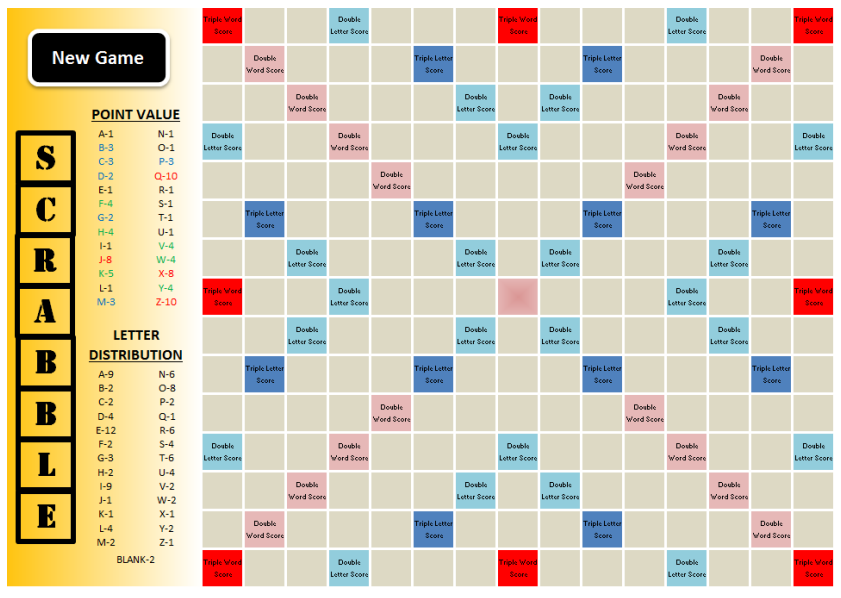
\includegraphics[width=0.65\paperwidth]{C:/Users/Admin/Desktop/Github/question_bank/LyX/static/img/9597-DHS-2015-P1-Q6-1}
\par\end{center}

Propose and justify
\begin{enumerate}
\item an efficient data structure to store the letter point values \hfill{}{[}3{]}
\item an efficient data structure to store the game board \hfill{}{[}3{]}
\item an efficient algorithm to compute the score of a word \hfill{}{[}4{]}
\end{enumerate}
{[}SPLIT\_HERE{]}
\end{enumerate}

\end{document}
